\section{Proposed method}\label{proposed-method}
\subsection{Background}
\subsubsection{Restricted Boltzmann Machine}

RBM model, a generative stochastic artificial neural network, is treated as a model in the field of deep learning.
RBM can be used to learn important aspects of an unknown probability distribution based on samples from this distribution~\cite{Fischer2012}.
Recently, researchers have applied RBM in the field of Natural Language Processing, including topic modeling and sentiment analysis~\cite{serbm}.
One special characteristic of RBM is that it can be used in both supervised and unsupervised ways, depending on the task.

As shown in Figure~\ref{fig:rbm1}, RBM model is a two-layer neural network which contains one visible layer and one hidden layer.
The visible layer is constituted by visible units correspond to the components of an observation (e.g., one visible unit for each word in an input document).
The hidden layer composed of hidden units which model the dependencies between the components of observations (e.g., dependencies between words in the document).

\begin{figure}
	\centering
	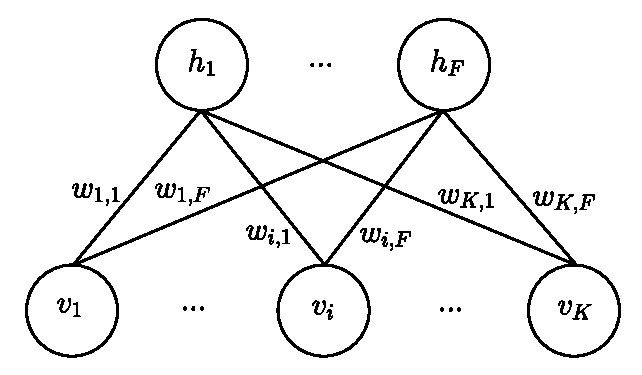
\includegraphics[height=3cm]{BasicRBM}
	\caption{The network graph of an RBM model with $K$ visible and  $F$ hidden units}
	\label{fig:rbm1}
\end{figure}

\subsubsection{Word Embedding model}

% Gioi thieu Word2Vec
The Word Embedding model (WEM) is a proven and powerful paradigm in Natural Language Processing, in which words are represented as vectors in a high-dimensional space~\cite{Quoc_Le}.
The idea of this model is representing words as vectors.
Therefore, the similarity of two words $i$ and $j$ can be calculated based on the cosine of the angle between the vectors as shown in equation~\ref{cosine_equal}.

\begin{equation} \label{cosine_equal}
\cos\theta=\frac{w_i.w_j}{||w_i|| ||w_j||}
\end{equation} 

where $w_i.w_j$ is the dot product of these two documents while $||w_i||$ and $||w_j||$ are the norm of vector $w_i$ and $w_j$, respectively.

% Mo rong Word2Vec thanh Doc2Vec
For document representation, every word appeared in the document is represented as a vector.
We then sum all of these vectors to get a vector that represent the document~\cite{Quoc_Le}.

\subsection{Our Aspect-based Sentiment Analysis model}
% Giới thiệu mô hình

\subsubsection{Structure}

% Research gap: fixed hidden unit
In the previous approach, Wang et al.~\cite{serbm} proposed an unsupervised RBM model to ABSA.
As mention before, there are two main shortcomings in this SERBM model.
%Although this model can help to overcome the limitations of hand-labeled training data, but there still exist certain shortcomings.
Firstly, an unsupervised method can only cluster reviews into categories and we can not know the name of the category.
This model fixes hidden units 0--6 to represent the target aspects \textit{Food}, \textit{Staff}, \textit{Ambience}, \textit{Price}, \textit{Ambience}, \textit{Miscellaneous}, and \textit{Other Aspects}, respectively.
%This may reduce the accuracy of the classification.
%Since unsupervised learning model can not fix the categories which it will cluster into the output units.
There is no way we can determine the aspects (e.g. which unit represents \textit{Food}, which unit represents \textit{Staff}) based on the position of the hidden units alone.

% Reseach gap: size of vector
Secondly, when training, each document is transformed into a $ \textit{K} \times \textit{D} $ matrix $\textbf{v}$, where $\textit{K}$ is the dictionary size, and $\textit{D}$ is the document length.
If visible unit $\textit{i}$ in $\textbf{v}$ takes the $\textit{k}$-th value, $v^k_i$ is set to 1.
If the training data has a large set of vocabulary, the visible layer will be a matrix combined by high-dimensional vectors.
These sparse input vectors lead to not only the decrease in the model's accuracy but also the increase in computational resources.

% Giải quyết research gap, sơ lược mô hình
To overcome these problems, we propose a method using supervised RBM model which is illustrated in Figure~\ref{fig:rbm2}.
The \textbf{\textit{Output units}} include the units represent the aspects and sentiment orientations of the reviews.
We call them \textit{Aspects identifying units} and \textit{Sentiments identifying units}, respectively.
These units are put together with \textbf{\textit{Input units}} in the visible layers, instead of being placed in hidden layers.
Meanwhile, the units in the hidden layer represent the relationship between the units in the visible layers.
We encode input units in the visible layer as a vector, created by the Word Embedding model~\cite{rehurek_lrec_word2vec}, instead the vector of one-hot encoding Bag Of Words model.
This helps reduce the dimensionality of the input matrix while keeping documents' semantics.

\begin{figure}
	\centering
	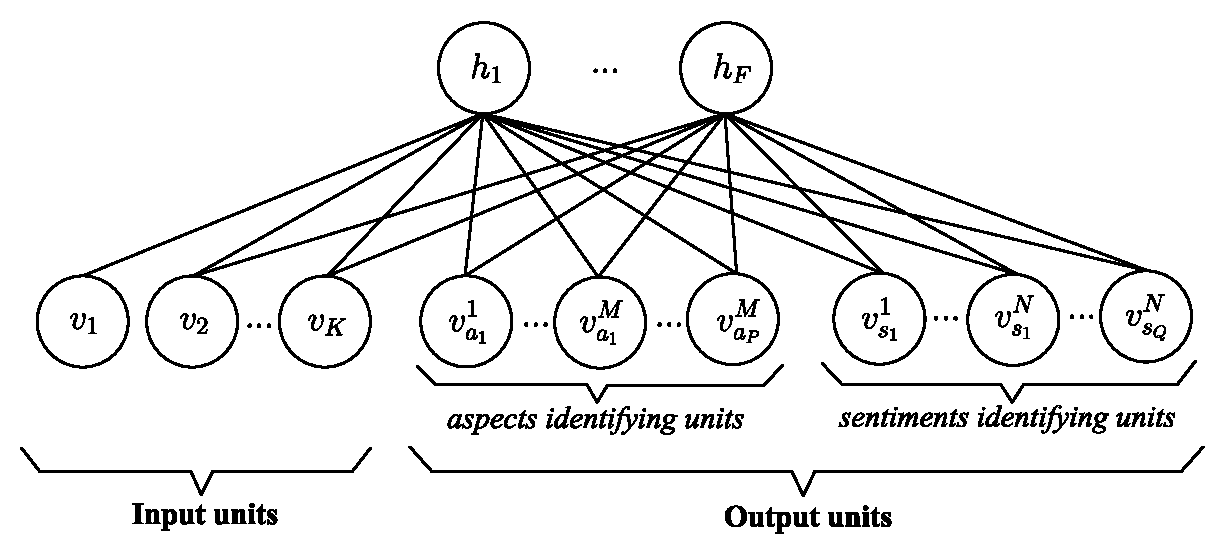
\includegraphics[height=4.5cm]{SupervisedRBM}
	\caption{The network graph of our Supervised Sentiment-Aspect Extraction RBM model}
	\label{fig:rbm2}
\end{figure}

% Nói chi tiết điểm khác biết giữa RBMs bình thường, chức năng mỗi node
Compared to standard RBMs, the first difference of this model is the visible layer.
Apart from the input units, there are also aspect and sentiment identifying units that represent the output component of the model.
Suppose in the training data, there are reviews talking about $P$ aspects and having $Q$ sentiment orientations in total.
In particular, the set of aspects is $ A = \{a_1, a_2, ..., a_P\}$, and the set of sentiment orientations is $ S = \{s_1, s_2, ..., s_Q\}$.

For each aspect, the model set $M$ units to capture that aspect.
For example, if the review mentioned aspect $a_i \in A$, we set the units from $v^1_{a_i}$ to $v^M_{a_i}$ to 1, and 0 otherwise.
We use the same setting for sentiment units.
The model set $N$ units to capture each sentiment polarity.
If the sentiment polarity is $s_j \in S$, we set the units from $v^1_{s_j}$ to $v^N_{s_j}$ to 1, and 0 otherwise.
The idea of setting M and N units to capture aspects and sentiment polarity is obtained from previous work~\cite{Fischer2012}.
Our model has the property that input units and output units stay in the same layer.
If we used only one output unit for each aspect and sentiment polarity while there are too many input units, the model would be imbalance and need more time to converge. 

% Nêu lý do tại sao lại chọn mô hình này
With this structure, our model can solve two tasks simultaneously: aspect identification and sentiment classification.
This ability of our model is reflected in the aspect and sentiment identifying units which play important roles in the sampling process of RBM.
Meanwhile, weight values of connecting edges contain semantic information of the review, which help identifying units to communicate with the hidden layer.
In addition, the fixed dimension of the input vector does not depend on the number of vocabulary words.
This capability not only helps the model prevent the occurrence of decreasing speed and accuracy, but also solves the semantic problem in the review.

For the customer restaurant reviews analyzing task, one word in a review may mention a certain aspect (e.g. ``delicious" corresponds to \textit{food} aspect), or a certain opinion (e.g. ``good" is about positive sentiment, while ``bad" is about negative sentiment).
Furthermore, there are other words do not mention about aspect or sentiment, they can be removed during the preprocessing phase.
These latent topics in a review are considered as the factors which generate aspect and sentiment words within that review.
To technically illustrate this, hidden layer contains information of the latent topics.
In the generation process, hidden units produce the values of visible units, which are also the information of the aspect and sentiment words in reviews.
Moreover, we can increase the number of hidden units in order to increase the modeling capacity of the RBM, which make the model powerful enough to represent complicated distributions.

\subsubsection{Word Embedding Restricted Boltzmann Machine}

% Những bất cập khi sử dụng chỉ word2vec mà không có prior knowledge
When we use supervised RBM with input vectors generated by Word Embedding model, the results showed that RBM does not have enough capacity to regenerate visible units.
Much of the instability in this approach stems from two reasons. 
Firstly, RBM has only hidden and visible layers to capture the diversity of semantic of documents.
Secondly, in visible and hidden units, the values vary continuously by each epoch in the training process.
This leads to loss of semantic information of documents.
One way to solve this problem is increasing the number of hidden units for RBM to accommodate more information.
However, increasing the number of hidden units causes the model to increase the number of visible units.
This leads to the problem encountered in the previous approach~\cite{serbm}, which is insufficient computational resources.

% Đề xuất thêm mô hình WE-RBM sử dụng prior knowledge
Therefore, we propose Word Embedding Restricted Boltzmann Machine (WE-RBM) to take full advantage of WEM's structure and supervised RBM.
Beside input units, WE-RBM also uses prior knowledge obtained from the vector comparing process of WEM.
Hence, the model would have more information to make up for the loss in the training process.
Our WE-RBM model is expressed in Figure~\ref{fig:vs-rbm}.

% Hình figure của WE-RBM
\begin{figure}
	\centering
	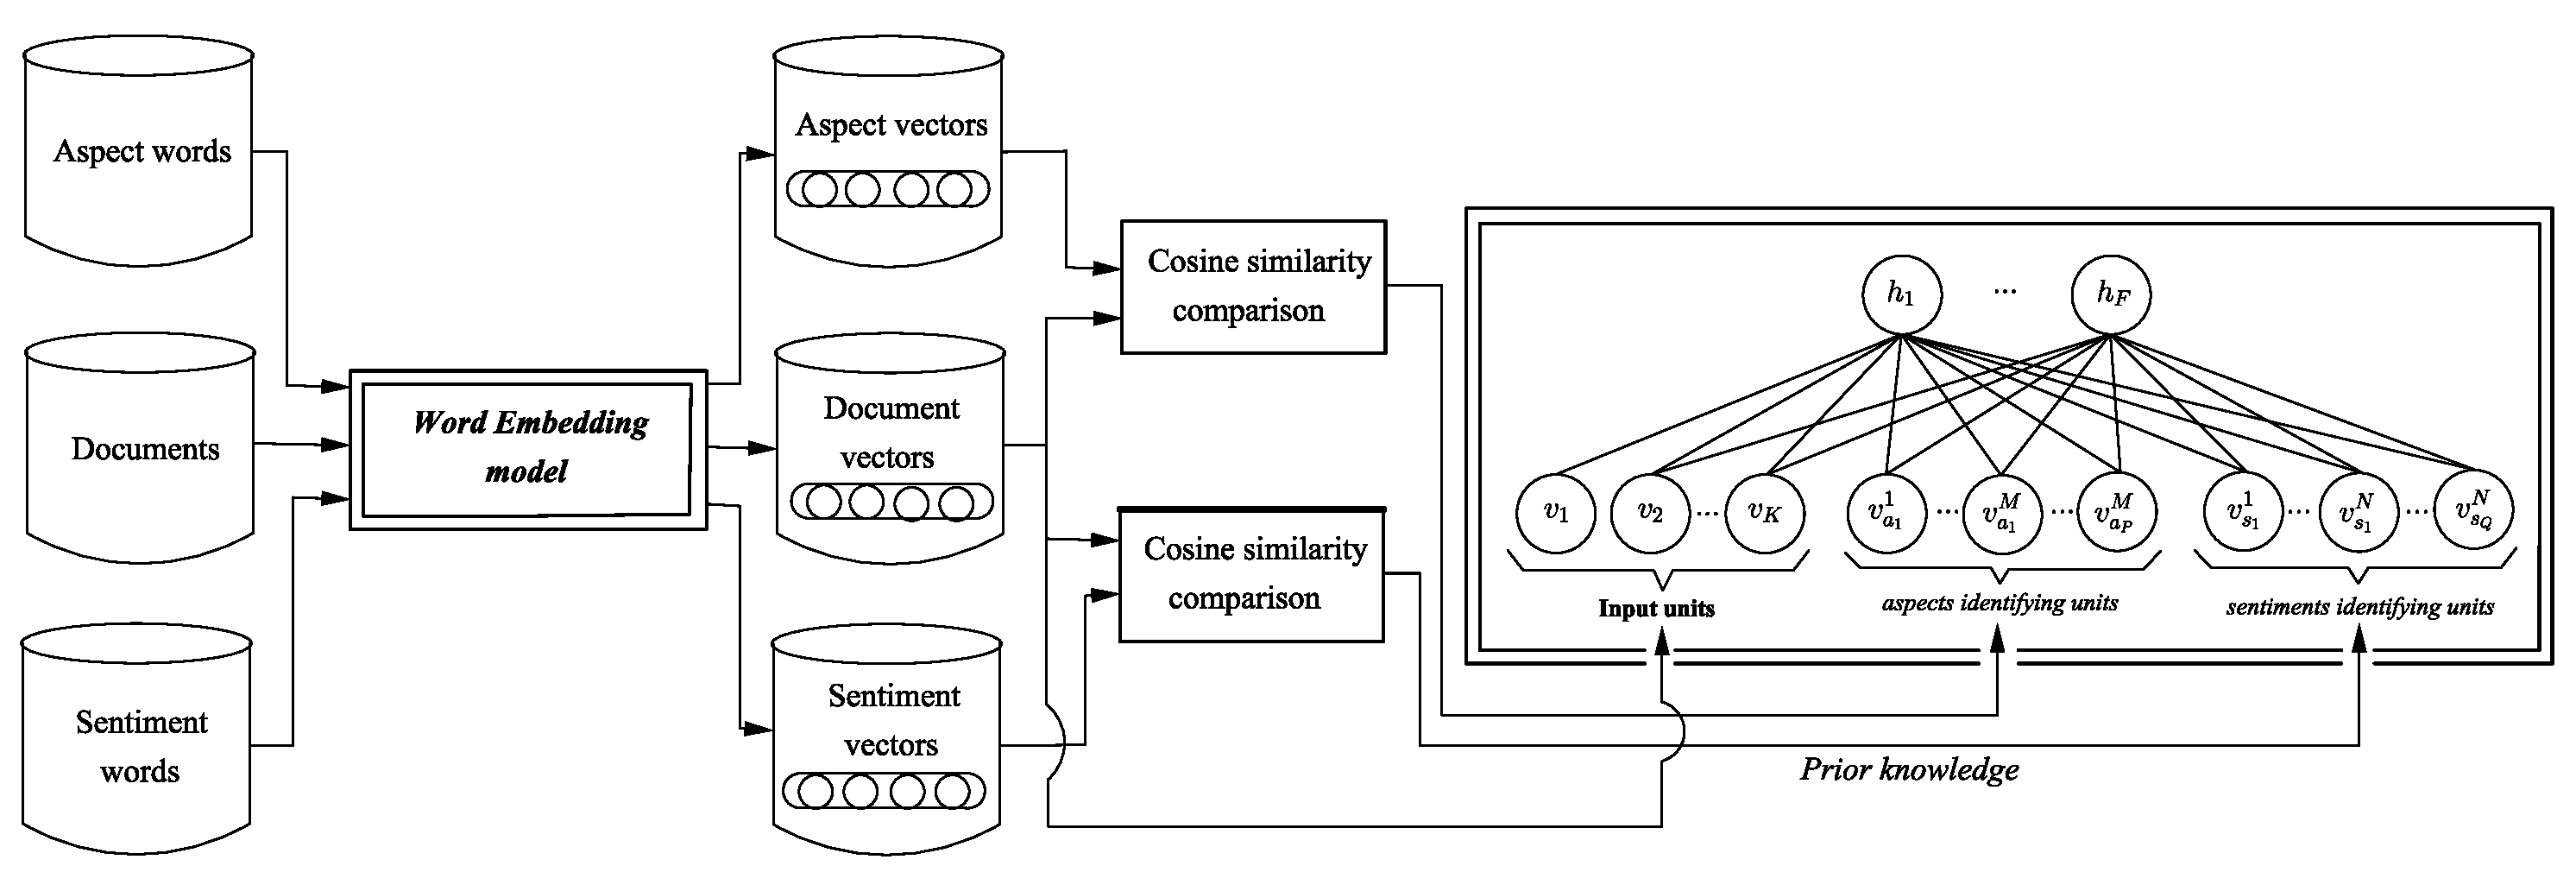
\includegraphics[height=4.0cm]{WE-RBM}
	\caption{WE-RBM model overview. Double boxed items are main components in WE-RBM model.}
	\label{fig:vs-rbm}
\end{figure}

% Giải thích figure
% Quá trình train
Assuming that WEM has been trained independently before, we put every document into WEM to generate the corresponding vector.
The dimension of each vector is equal to the number of input units of RBM.
After document vectors generation process, we make the training phase for the RBM model in a supervised setting.
This phase helps the model be able to understand the vectors' pattern generated by WEM.

% Trong quá trình test
In the testing phase, each document is also converted into a vector by WEM.
Unlike previous work, the aspect identification and sentiment classification task are firstly performed by WEM instead of RBM model.
Particularly, WE-RBM computes the cosine similarity score (shown in equation \ref{cosine_equal}) between the document vector and each of all aspect and sentiment vectors, which are also generated by WEM.
The prior knowledge is determined by the highest similar pair of vectors.

For instance, a document $d$ can be categorized into one of these aspects $S = {a_1, a_2,..., a_P}$.
Let us call the vector form of document or aspect $x$ $vec(x)$.
Prior knowledge would be labeled $i$ if cosine similarity between $vec(d)$ and $vec(a_i)$ is the highest one.
The model performs similarly with sentiment classification task.
This prior knowledge can help improve the ability of the model to extract aspects and identify sentiments.
 
% Lý do có được ý tưởng này
One characteristic of WEM is two vectors which represent two different words would have high cosine similarity if these two words have close meaning to each other~\cite{rehurek_lrec_word2vec,Milokov_word2vec} (e.g. ``strong" may have close meaning with ``powerful", whereas ``strong" and ``London" are more distant).
Inspired by this, we use WEM to categorize aspect and classify sentiment before feeding the input vector into RBM model.
Hence, each document can have its own prior knowledge before RBM's classification.
The final classification result is determined by both WEM and RBM.
Therefore, we call our novel combination model is WE-RBM.

% Giải thích tại sao lựa chọn mô hình này, lợi ích của mô hình
There are three main reasons we propose this novel WE-RBM model to solve the ABSA's tasks.
Firstly, when a document is converted into vector form, it can be compared with other documents by cosine similarity while semantic information is conserved.
This is the advantage of word representation technique that WE-RBM use in the classification process.
Secondly, WE-RBM can save computational resources and processing time.
The model does not need to adapt input units for huge dictionary size thanks to fixed dimension of the input vector.
Using prior knowledge instead of increasing hidden units, WE-RBM can handle big training set in reduced processing time.
Last but not least, our WE-RBM model also has the capability of jointly modeling aspect and sentiment information together.

\subsubsection{Training and Testing}
% Mô tả quá trình huấn luyện của mô hình
In the training process, Contrastive Divergence (CD), also called Approximate Gradient Descent, is the way that helps RBM learn the connection weights in the network.
CD has two phases, which are Positive phase and Negative phase.
In each phase, we compute the positive and negative value by the multiplication of visible and hidden units.
Then, we update the connection weight based on the subtraction from positive value of negative value.
Particularly, each epoch of CD can be expressed in five steps below:

\textbf{\emph{Step 1}}.
Update the states of the hidden units using the logistic activation rule described in equation~\ref{equation:vtoh}.
For the $j$-th hidden unit, compute its activation energy and set its state to 1 with corresponding probability.
\begin{equation} \label{equation:vtoh}
P(\emph{h}_j=1| \textbf{v})=sigm(a_j+\sum^D_{i=1}\sum^K_{k=1}v^k_iW^k_{ij})
\end{equation}

\textbf{\emph{Step 2}}.
For each connection edge $e_{ij}$, get the value from positive phrase by equation~\ref{pos_phrase}.
\begin{equation} \label{pos_phrase}
pos(e_{ij}) = v_ih_j
\end{equation}

\textbf{\emph{Step 3}}.
Reconstruct the visible units in a similar manner by using the logistic activation rule described in equation~\ref{equation:htov}.
For the $i$-th visible unit, compute its activation energy and set its state to 1 with corresponding probability.
Then do \textbf{\emph{Step 1}} to update the hidden units again.
\begin{equation} \label{equation:htov}
P(v_i^k=1| \emph{h})=sigm(b_i^k+\sum^F_{j=1}h_jW^k_{ij})
\end{equation}

\textbf{\emph{Step 4}}.
For each connection edge $e_{ij}$, get the value from negative phrase by by equation~\ref{neg_phrase}.
\begin{equation} \label{neg_phrase}
neg(e_{ij}) = v_ih_j
\end{equation}

\textbf{\emph{Step 5}}.
Update the connection weights $W_{ij}$ by equation~\ref{update_w}.
\begin{equation} \label{update_w}
W_{ij} = W_{ij}+\textbf{lr}(pos(e_{ij}) - neg(e_{ij}))
\end{equation} 
where  $sigm(x) = \frac{1}{(1+e^{-x})}$ is the logistic function, and $\textbf{lr}$ is a learning rate. 

After $m$ epochs of transfer between visible and hidden layers in a CD-$m$ run of the above steps, values of the hidden units reflect the relationship between the visible units in the model.
The connection weight matrix between the two layers helps hidden layer generate visible units which include input units, aspect identifying units and also sentiment identifying units.

% Mô tả quá trình kiểm thử (thêm phần tiền phân lớp bằng prior probability)
In the testing process, we convert all documents into vector form using WEM.
Then, each document vector is compared with each aspect vector by cosine similarity score.
The most similar pair of vectors gives the model prior knowledge about the aspect label of this document.
Final aspect label of the document is determined based on the result of aspects identifying units after WE-RBM generation process.